\documentclass[12pt,a4paper]{article} 

\usepackage[utf8]{inputenc}
\usepackage[margin=1.3cm]{geometry}
\usepackage[francais]{babel} 
\usepackage{amsfonts} 
\usepackage{graphicx} 
\usepackage{amsmath} 
\setlength{\unitlength}{1mm}
\usepackage{enumitem}
\usepackage{cancel}
\usepackage{fancyhdr}
\usepackage{fancybox}
\usepackage{hyperref}
\usepackage{array}
\usepackage{titling}
\usepackage{stmaryrd}
\usepackage{graphicx}
\usepackage{wrapfig}
\usepackage{algorithm}
\usepackage{algpseudocode}
\graphicspath{ {./images/} }
\usepackage{graphicx} % taille des tableaux
\usepackage{multirow} % tableaux
\usepackage[justification=centering]{caption}
\usepackage{lastpage}

\DeclareMathOperator*{\argmax}{argmax}
\DeclareMathOperator*{\argmin}{argmin}

\makeatletter
\renewcommand{\ALG@name}{Algorithme}

\algblock{Input}{EndInput}
\algnotext{EndInput}

\cfoot{\thepage\ / \pageref{LastPage}}

\author{Antoine Groudiev - n°15039}
\date{\vspace{-6ex}}
\title{\textit{Rapport de synthèse du TIPE :} \\ Vision par ordinateur appliquée à la détection de panneaux}

\begin{document}
\maketitle

\section*{Introduction}
La détection d'objets est la branche de la vision par ordinateur visant à classifier des images selon la présence ou l'absence d'un objet spécifique dans l'image. Je me suis intéressé à la détection de panneaux routiers dans un flux vidéo, et plus spécifiquement à un algorithme de \textit{boosting}. Le terme \textit{boosting} désigne une famille d'algorithmes d'apprentissage qui pondère un ensemble de classificateurs faibles, qui classent chacun légèrement mieux que le hasard, pour former un classificateur fort de bonne exactitude.

\section{Algorithme de Viola et Jones}
\textit{AdaBoost} est un des algorithmes de \textit{boosting} les plus populaires, notamment grâce à son utilisation par la méthode de Viola et Jones, un algorithme de reconnaissance de visages, présenté en 2001 \cite{viola-jones}.

Le détecteur doit pouvoir prendre en entrée des images de tailles quelconques, et retourner la liste des emplacements dans l'image de l'objet à détecter. La première phase de la création du détecteur se restreint cependant à la détection d'objets dans une image carrée de petite taille : j'ai fait le choix de \texttt{19px} de côté. La dernière partie de l'algorithme, détaillée en \ref{sec:taille_standard}, appliquera ce détecteur à une image detaille standard, i.e. de plusieurs centaines de pixels de côté.

\subsection{Classificateurs faibles}
Les algorithmes de \textit{boosting} fonctionnent par sélection de classificateurs faibles. Dans le contexte de la méthode de Viola et Jones, un classificateur faible est constitué de trois éléments.

\subsubsection{Les \textit{features}}

\begin{wrapfigure}{r}{0.4\textwidth}
    %\begin{figure}[h]
        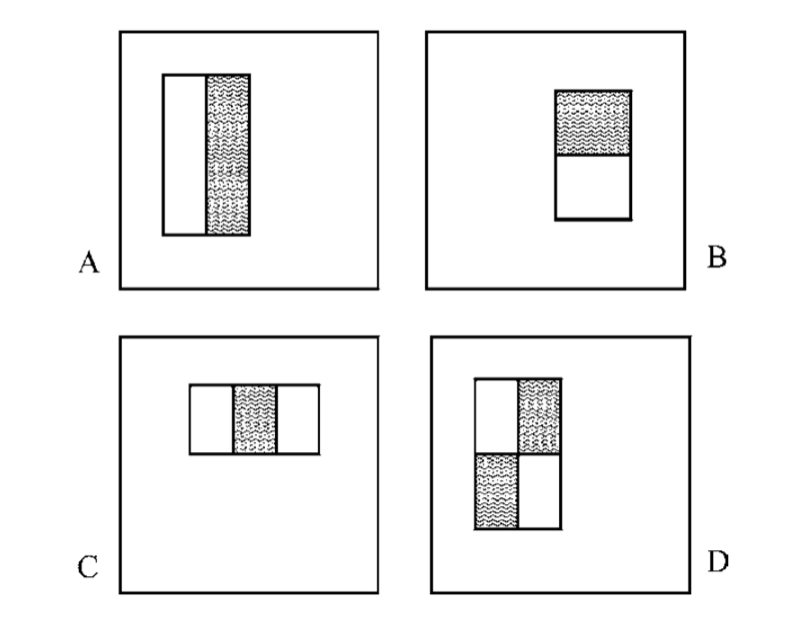
\includegraphics[scale = 0.4]{forme_features}
        \centering
        \caption{Forme des \textit{features}}
        \label{fig:forme-features}
    %\end{figure}
\end{wrapfigure}
    
Une \textit{feature} est consitutée de $2$ à $4$ régions rectangulaires adjacentes, comptées positivement ou négativement. Leurs formes sont imposées comme dans la \autoref{fig:forme-features}. 
Chaque \textit{feature} va cibler une zone spécifique de l'objet à détecter. Dans le cas d'un visage par exemple, le détecteur peut apprendre que la zone du creux de l'œil est généralement plus sombre que la zone entre les deux yeux. Ainsi, une image comportant cette différence de luminosité caractéristique sera probablement un visage.


Le score d'une \textit{feature} $f$ peut être évalué sur une image $x$ à l'aide de la formule suivante (le score le plus faible en valeur absolue étant le meilleur) :

\begin{equation}\label{score-feature}
    f(x) = \sum_{r \in R_+} r(x) - \sum_{r \in R_-} r(x)
\end{equation}

où $r(x)$ désigne la somme des pixels dans la région délimitée par $r$. Une méthode efficace du calcul de $r(x)$ sera donnée par l'équation \ref{somme-region}. Intuitivement, la formule \ref{score-feature} traduit que le score d'une \textit{feature} est d'autant plus faible que les zones positives compensent les zones négatives. 


Le nombre de \textit{features} possibles croît exponentiellement avec le côté de l'image, d'où la nécessité d'entraîner dans un premier temps un détecteur de côté faible.

\begin{wrapfigure}{r}{0.4\textwidth}
%\begin{figure}[h]
    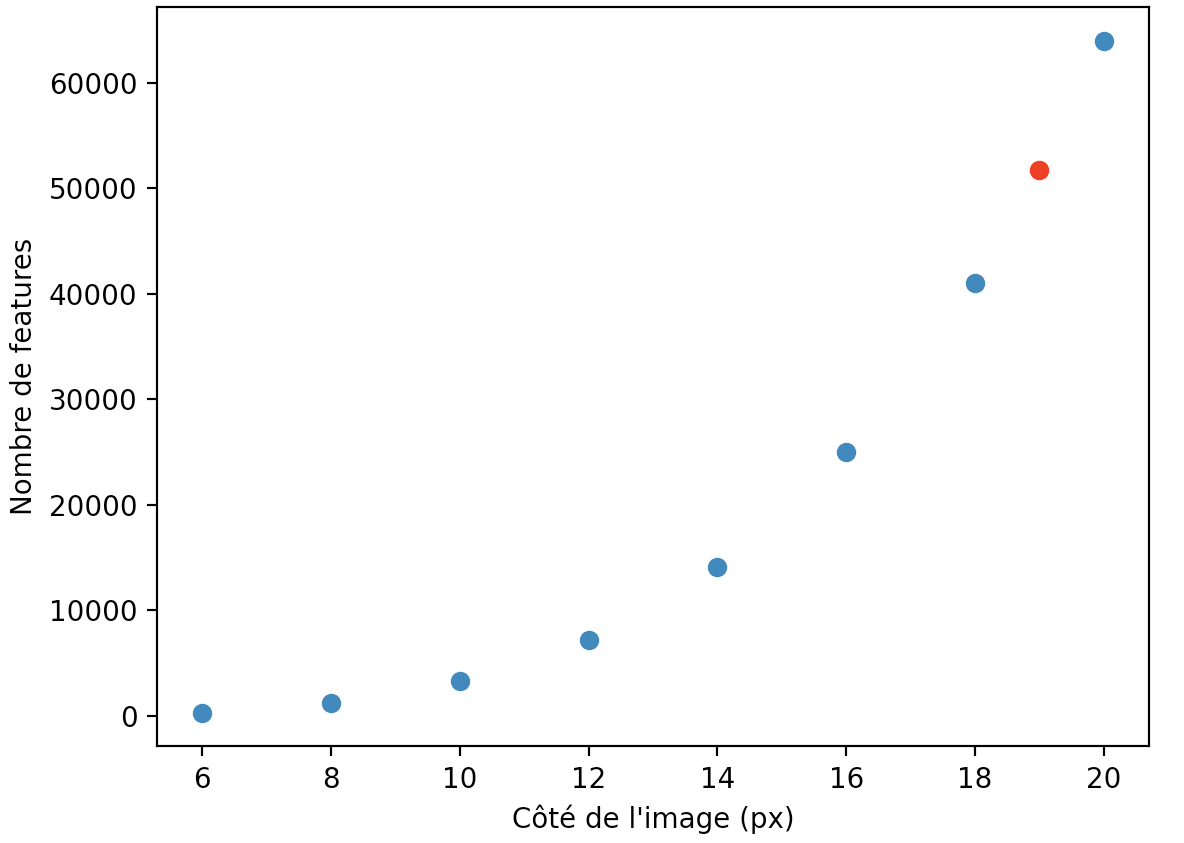
\includegraphics[scale = 0.35]{nombre_features_cut}
    \centering
    \caption{Nombre de \textit{features} en fonction de la taille de l'image}
%\end{figure}
\end{wrapfigure}

\subsubsection{Évaluation par un classificateur faible}
À chaque \textit{feature} (notée $f$) est associée un \textit{threshold} (ou seuil) $\theta > 0$, et une polarité $p \in \{-1 ; 1\}$. Soit $x$ une image de \texttt{19px} de côté. Le classificateur faible $C_{(f, \: \theta, \: p)}^{faible}$ convertit le score de la \textit{feature} sur $x$ en un booléen selon la loi suivante :

\begin{equation}
    C_{(f, \: \theta, \: p)}^{faible}(x) = 
        \begin{cases}
        1 \:\: si \:\: pf(x) < p\theta \\
        0 \:\: sinon
        \end{cases}
\end{equation}

Si le score de la \textit{feature} sur $x$ est, à la polarité près, sous le seuil, alors le classificateur faible juge que la zone de l'image correspond à l'objet à détecter.

\subsection{Image intégrale}
La complexité du calcul du score d'un classificateur faible est déterminée par la complexité du calcul de la somme des valeurs des pixels dans un sous-rectangle de l'image.

Une approche naïve consisterait à recalculer, à chaque évaluation du score d'un classificateur, la somme des valeurs des pixels de l'image dans certaines de ses régions rectangulaires. Un tel calcul pour une région de taille $L_r$ sur $l_r$ a une complexité en $O(L_r \times l_r)$. Si l'on considère une image de dimensions $n \times n$ et que l'on veut calculer la somme dans $p$ régions de dimensions proches de $n \times n$, la complexité totale est en $O(p \times n^2)$.

\begin{wrapfigure}{l}{0.4\textwidth}
    %\begin{figure}[h]
        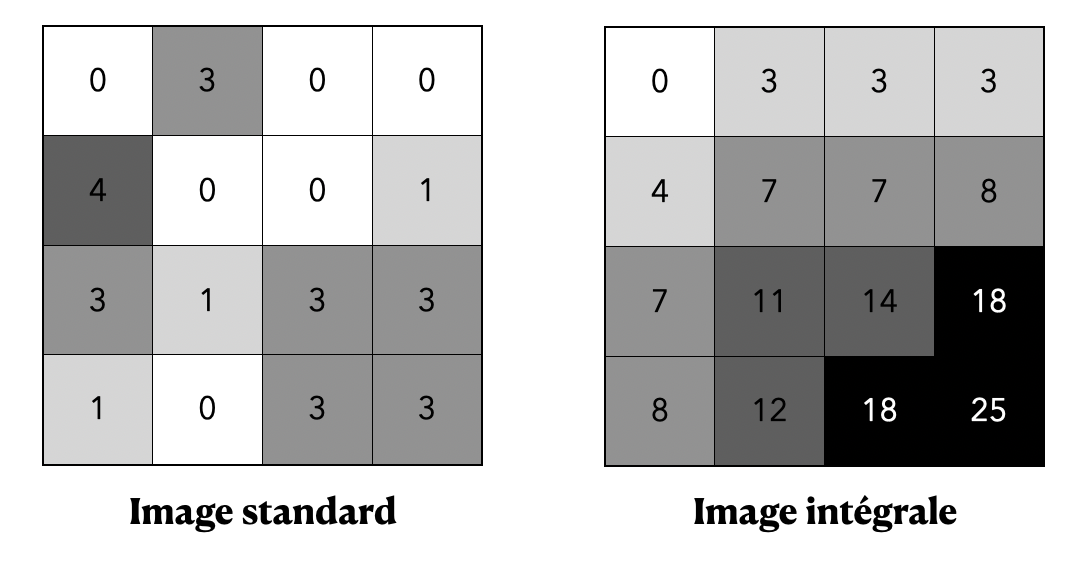
\includegraphics[scale = 0.35]{image-integrale2}
        \centering
        \caption{Exemple d'image intégrale}
    %\end{figure}
    \end{wrapfigure}

Pour réduire cette complexité, la méthode de Viola et Jones introduit \textbf{l'image intégrale}. Si l'image considérée est $(i(x, y))$, alors l'image intégrale, notée $(ii(x, y))$ vérifie :

\begin{equation}
    \forall x, y, ii(x, y) = \sum_{x' \leq x, y' \leq y} i(x', y')
\end{equation}

Ainsi, chaque coefficient de l'image intégrale contient la somme des coefficients en haut à gauche du pixel considéré. Ceci permet alors d'accéder en temps constant à la somme des pixels dans un sous-rectangle de l'image $(i(x, y))_{x, y}$, en réalisant simplement la somme de quatre termes. En effet, considérons $R$ le sous-rectangle délimité par les sommets $(x_1, y_1)$ et $(x_2, y_2)$. Alors la somme $r(x)$ des pixels de l'image $x$ dans la région $R$ vaut :

\begin{equation}\label{somme-region}
    r(x) = ii(x_2, y_2) - ii(x_2, y_1) - ii(x_1, y_2) + ii(x_1, y_1)
\end{equation}


\subsection{Sélection des caractéristiques par \textit{AdaBoost}}
La phase de \textit{boosting} à proprement parler vise à sélectionner un nombre $T \in \mathbb{N}^*$ de classificateurs faibles qui représentent le mieux l'objet à détecter. L'algorithme utilise pour cela en entrée un jeu d'entraînement, c'est-à-dire une liste de tuples $(x, y) \in \mathcal{M}_{19, 19}(\llbracket 0, 255 \rrbracket) \times \{0 ; 1\}$. 

Chaque tuple est constitué d'une image contenant ou ne contenant pas l'objet à détecter, centré et cadré le cas échéant, et d'un label booléen, valant $1$ si l'objet à détecter est effectivement représenté sur l'image. La constitution d'un tel jeu sera détaillée dans la Partie \ref{sec:pre-traitement}.

\begin{figure}[h]
    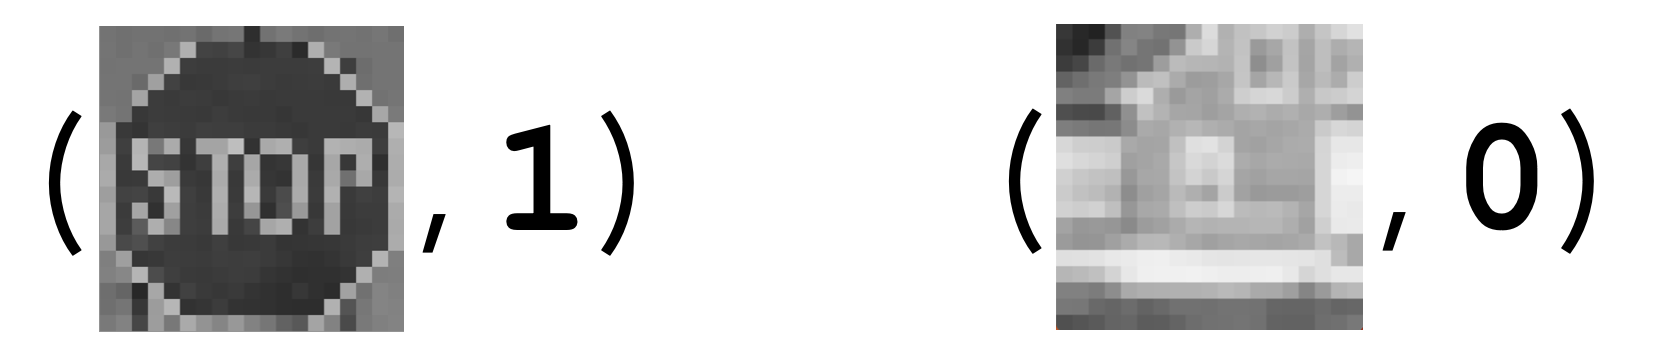
\includegraphics[scale = 0.4]{exemples-jeu-cut}
    \centering
    \caption{Exemple de deux tuples du jeu d'entraînement}
\end{figure}

L'algorithme \textit{AdaBoost} est un algorithme glouton qui sélectionne un à un les $T$ meilleurs classificateurs parmi les $50\,000$ présents dans l'image de \texttt{19px} de côté. Son initialisation consiste en l'affection à chaque image d'un poids, qui équilibre l'importance des images positives et négatives. Ensuite, la sélection d'un classificateur se fait en trois grandes étapes : l'erreur de chaque classificateur est calculée selon le classement qu'il fait de chaque image et de leurs poids respectifs ; le classificateur d'erreur minimale est sélectionné ; les poids sont mis à jours pour prendre en compte le nouveau classificateur, puis normalisés.

%\begin{wrapfigure}{L}{0.6\textwidth}
%\begin{minipage}{0.6\textwidth}
\begin{algorithm}[H]
    \caption{Entraînement par AdaBoost}
    \begin{algorithmic}
        \Input

        $(x_1, y_2), ..., (x_n, y_n)$
        \Comment{Jeu d'entraînement}
        \EndInput
        \State $m \gets$ nombre d'images négatives
        \State $l \gets$ nombre d'images positives
        \For{$i \in \llbracket 1, n \rrbracket$} \Comment{Initialisation des poids}

            \State $w_{1, i} \gets \begin{cases}
                \frac{1}{m} \:\: si \:\: y_i = 0 \\
                \frac{1}{l} \:\: sinon
                \end{cases}$
        \EndFor
        \For{$t \in \llbracket 1, T \rrbracket$}

            \For{$i \in \llbracket 1,$ nombre de classificateurs $\rrbracket$}

                \State $\varepsilon_i = \sum_i w_{t,i} \times \delta(C_i^{faible}(x_i), \overline{y_i})$ \Comment{Calcul de l'erreur de chaque classificateur}
            \EndFor

            \State $C_t^{faible} \gets \argmin_{C_i^{faible}} \varepsilon_i$
            \For{$i \in \llbracket 1, n \rrbracket$} \Comment{Mise à jour des poids}

            \If{image $x_i$ bien classée par $C_t^{faible}$}
                \State $w_{t+1, i} \gets w_{t, i} \times \frac{\varepsilon_t}{1- \varepsilon_t}$ \Comment{le poids baisse à $t+1$}

            \Else
                \State $w_{t+1, i} \gets w_{t, i}$ \Comment{le poids augmente à $t+1$}
            \EndIf

            \EndFor
            \State Normaliser les poids : $w_{t, i} \gets \frac{w_{t, i}}{\sum_{j=1}^n w_{t, j}}$
        \EndFor
    \end{algorithmic}
\end{algorithm}
%\end{minipage}
%\end{wrapfigure}

En toute généralité, la complexité de \textit{AdaBoost} est en $O(n \cdot F \cdot \tau + T \cdot n)$ où $n$ désigne le nombre d'images d'entraînement, $F$ le nombre total de classificateurs faibles, et $\tau$ le temps moyen de classification d'un classificateur faible sur un $x_i$. On a $T = O(F)$ et dans le cas de Viola-Jones, l'image intégrale garantit $\tau = O(1)$, ce qui donne une complexité en $O(n \cdot F)$.

Après sélection des $T$ classificateurs faibles, l'algorithme les combine en un unique classificateur fort $C^{fort}$, défini par :

\begin{equation}
    C_T^{fort}(x) = 
    \begin{cases}
    1 \:\: si \:\: \sum_{i=1}^T \alpha_i C_i^{faible}(x) \leq \frac{1}{2} \sum_{i=1}^T \alpha_i \\
    0 \:\: sinon
    \end{cases}
\end{equation}

où les $\alpha_i = \log(\frac{1 - \varepsilon_i}{\varepsilon_i})$ pondèrent les classificateurs selon leur erreur. Ainsi, aux pondérations près, si au moins la moitié des classificateurs faibles retournent $1$, le classificateur fort retourne $1$.


\subsection{Mise en cascade}
Selon sa valeur de $T$, un classificateur fort est soit très efficace (pour $T$ faible), soit très exact (pour $T$ élevé). L'introduction du concept de cascade permet d'allier exactitude et efficacité. 

\begin{figure}[h]
    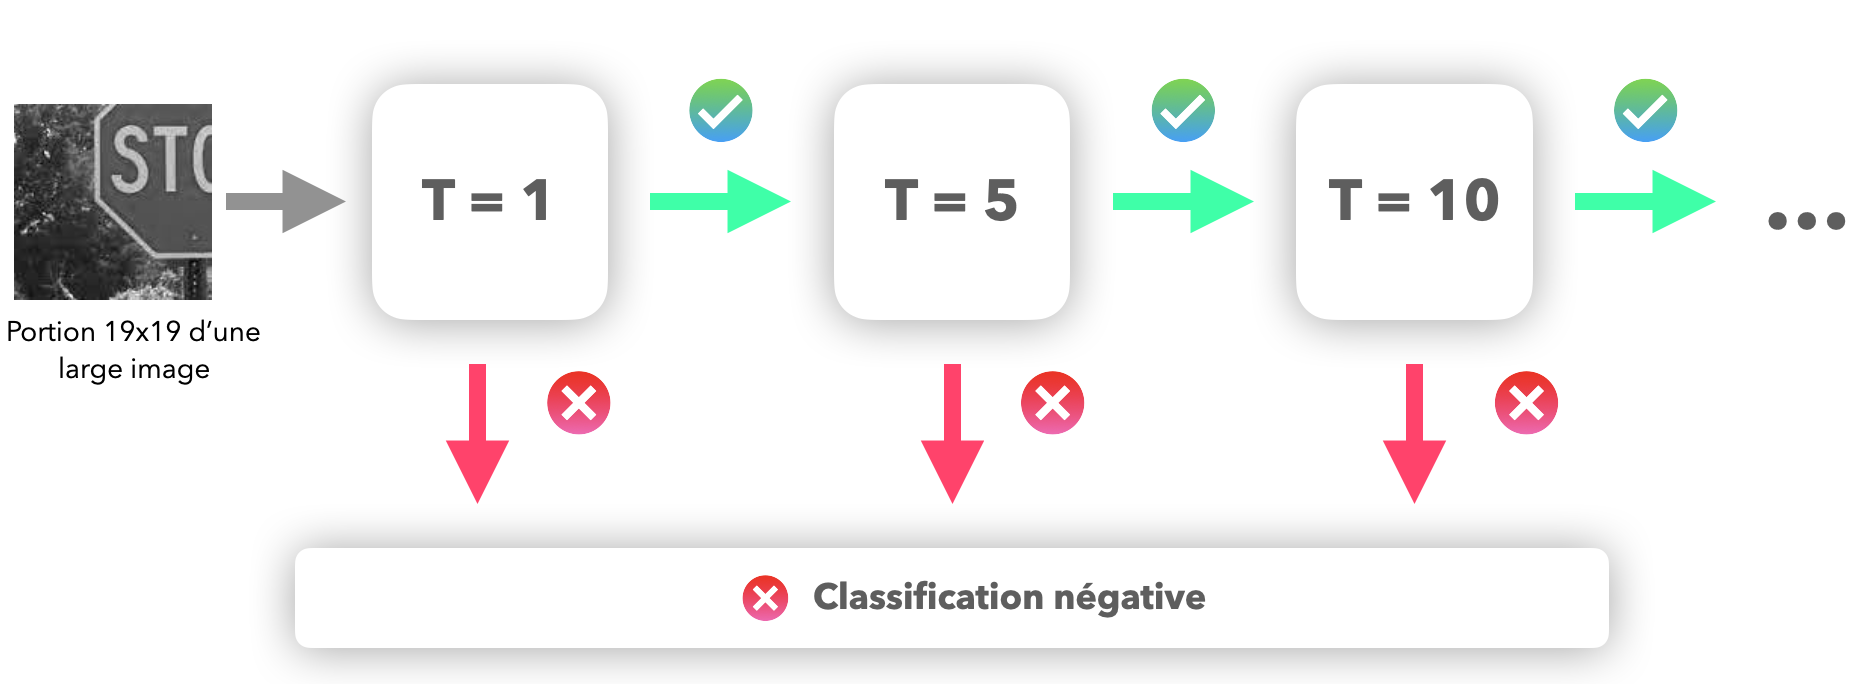
\includegraphics[scale = 0.4]{cascade}
    \centering
    \caption{Schéma d'une cascade}
\end{figure}

Une image analysée par la cascade va être classée successivement par une suite $(C_T^{fort})_T$ pour des valeurs de $T$ croissantes. Une image est alors rejetée par la cascade dès qu'elle est classée négativement par un des classificateurs forts, permettant une grande efficacité. Au contraire, une image finalement classée positivement par la cascade sera passée à travers des classificateurs forts avec $T$ très grands, garantissant un faible nombre de faux positifs.

\subsection{Application à des images de taille standard}
\label{sec:taille_standard}
L'application du détecteur à une image standard se fait en analysant des sous-fenêtres carrées de la grande image. 

\begin{figure}[h]
    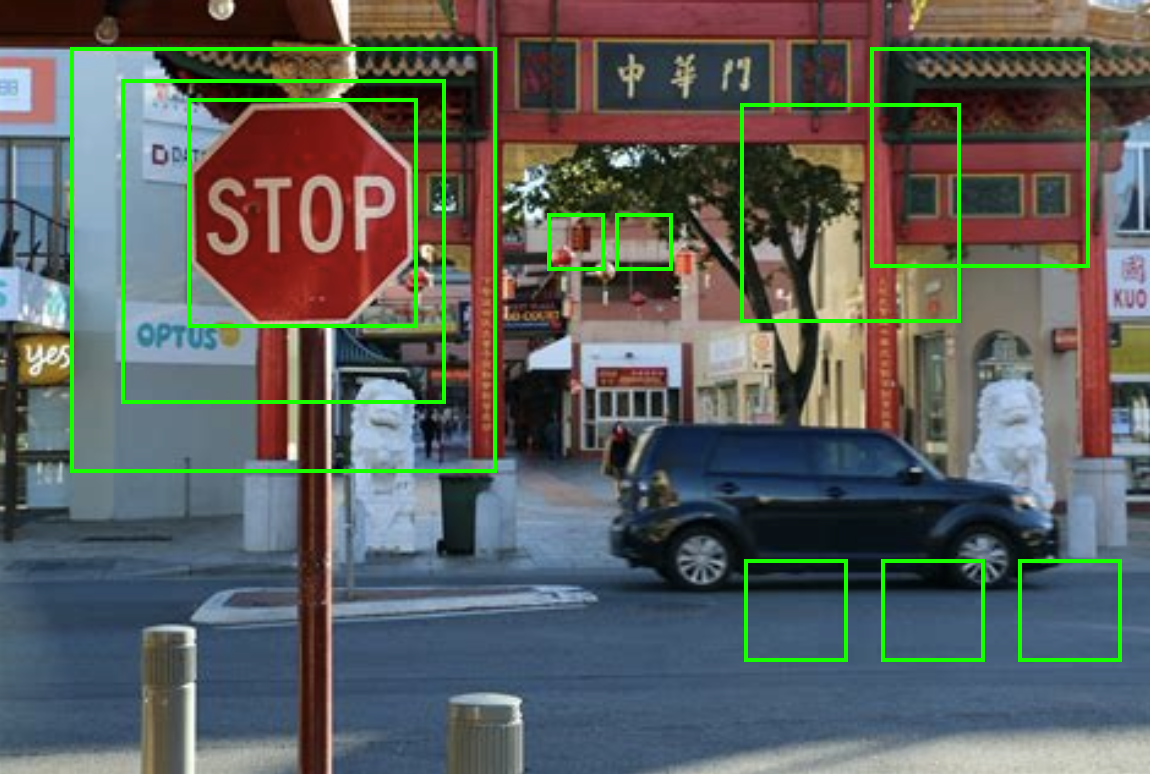
\includegraphics[scale = 0.5]{sous-fenetre}
    \centering
    \caption{Exemples de sous-fenêtres d'une image de taille standard}
\end{figure}

Le détecteur ne pouvant analyser l'intégralité des millions de sous-fenêtres de l'image, l'analyse est déterminée par deux paramètres : le paramètre $\Delta$, décalage entre deux sous-fenêtres de même taille, et le paramètre $s$ (pour \textit{scaling}), rapport des tailles de deux sous-fenêtres de côtés différents.

Le choix de ces deux paramètres permettra de contrôler la relation entre exactitude et efficacité du détecteur, commme observé dans les résultats de la Partie \ref{sec:results-standard}.

\section{Pré-traitement des images d'entaînement et de test}
\label{sec:pre-traitement}
Viola et Jones ont utilisé pour l'entraînement de leur algorithme une base de données constituée de $4916$ images positives et $9544$ images négatives. Le nombre d'images positives a même été doublé en introduisant les symétriques verticaux, ce qui est impossible dans mon cas en raison de l'asymétrie de la plupart des panneaux. 

Une telle quantité d'images n'existe pas pour l'objet sur lequel je me suis concentré, le panneau STOP, ce qui a naturellement une influence sur les résultats de mon implémentation. J'ai pû réunir $400$ images de panneaux STOP, que j'ai pré-traitées avant d'entraîner le détecteur.

\begin{figure}[h]
    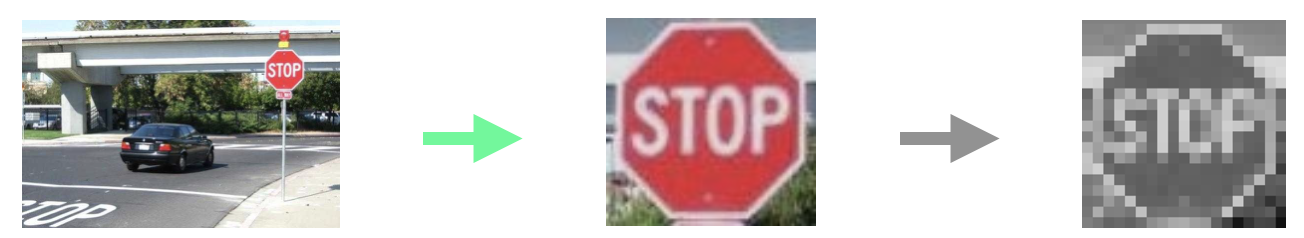
\includegraphics[scale = 0.5]{traitement}
    \centering
    \caption{Étapes du pré-traitement d'une image}
\end{figure}

La première étape consiste en un recadrage manuel de l'image. La seconde, réalisée par un script, redimensionne l'image vers \texttt{19px} de côté par interpolation bilinéaire, et la convertit en niveaux de gris, chaque pixel appartenant finalement à $\llbracket 0, 255 \rrbracket$ (\texttt{8 bits}).

\section{Mesure de l'exactitude et de l'efficacité de l'implémentation}
Le langage courant confond l'exactitude, c'est à dire la proximité du résultat expérimental à la valeur théorique, et la précision, qui quantifie la dispersion des résultats. L'objectif de cette dernière partie vise à déterminer précisément l'exactitude du détecteur précédement implémenté.

\subsection{Quantification de l'exactitude}
Toute quantification de l'exactitude est une expression des coefficients de la \textbf{matrice de confusion} d'un détecteur, matrice qui compare le classement du détecteur au label réel.

\begin{wrapfigure}[7]{r}{0.4\textwidth}
    \renewcommand{\arraystretch}{1.5}
    \begin{tabular}{|c|c|c|}
        \cline{2-3}
        \multicolumn{1}{c|}{} & \textbf{Classé : P} & \textbf{Classé : N} \\
        \hline
        \textbf{Réel : P} & $V_p$ & $F_n$ \\
        \hline
        \textbf{Réel : N} & $F_p$ & $V_n$ \\
        \hline
    \end{tabular}
    \caption{Matrice de confusion}
    \label{fig:matrice-confusion}
\end{wrapfigure}

%\begin{enumerate}
%    \item $V_p$, le nombre de vrais positifs
%    \item $V_n$, le nombre de vrais négatifs
%    \item $F_p$, le nombre de faux positifs
%    \item $F_n$, le nombre de faux négatifs
%\end{enumerate}

\subsubsection{Approche standard}
Il semble intuitif de poser l'exactitude comme étant :
\[
    A = \frac{bons\ classements}{total} 
\]
Ou encore avec les notations de la \autoref{fig:matrice-confusion} :
\begin{equation}
    \boxed{A = \frac{V_p + V_n}{V_P + V_n + F_p + F_n}}
\end{equation}

Cependant, cette méthode de calcul introduit des biais en cas de déséquilibre important entre le nombre d'images positives et le nombre d'images négatives. Nos échantillons de tests étant fortement déséqulibrés, il faut introduire une nouvelle méthode de calcul de l'exactitude.

\subsubsection{F-Score}
On introduit alors souvent le F-Score ou $F_1$-Score, défini comme la moyenne harmonique de la précision et du rappel. \cite{powers}

La précision et le rappel sont définis comme :
\begin{equation}
    P = \frac{bons\ classements}{classements\ positifs} = \boxed{\frac{V_p}{V_P + F_p}}
    \hspace{5em}
    R = \frac{bons\ classements}{images\ positives} = \boxed{\frac{V_p}{V_P + F_n}}
\end{equation}

Finalement, le F-Score est donnée comme la moyenne harmonique des deux :
\begin{equation}
    \boxed{F_1 = \frac{2}{\frac{1}{P} + \frac{1}{R}} = \frac{2 P R}{P+R}}
\end{equation}


\subsection{Résultats du détecteur de \texttt{19px}}
Après entraînement sur un jeu d'images de panneaux STOP, j'ai obtenu les résultats suivants :
\renewcommand{\arraystretch}{1.3}
\begin{table}[h]
    
    \resizebox{1.05\textwidth}{!}{
    \centering{
    \begin{tabular}{|c||c|c||c|c||c|}
        \hline
        $T$ par couche & Jeu d'entraînement & Jeu de test & Exactitude (standard) & Exactitude (F-Score) & Temps moyen de classification \\
        \hline
        \hline

        1, 5, 10 & \multirow{2}{*}{324 / 4548 / 1:14} & \multirow{2}{*}{69 / 3450 / 1\!:50} & 96,7 \% & 81,3 \% & 0,633 ms \\

        \cline{1-1} \cline{4-6}

        1, 5, 10, 20, 50 &  &  & 98,6 \% & 91,5 \% & 0,696 ms \\

        \hline
    \end{tabular}
    }
}
\end{table}

On remarque que l'augmentation du nombre de couches du détecteur dans la seconde ligne améliore l'exactitude du détecteur, au coût d'un temps moyen de classification plus élevé. Le temps de classification est néanmoins loin d'être linéaire en le nombre total de classificateurs faibles, ce qui est logique puisque seules les images positives prennent sensiblement plus de temps à être traitées.

\subsection{Résultats du détecteur de taille standard}
\label{sec:results-standard}
J'ai par la suite testé mon détecteur sur des images de taille standard, et ai obtenu les résultats suivants :
\renewcommand{\arraystretch}{1.3}
\begin{table}[h]
    
    \resizebox{1.05\textwidth}{!}{
    \centering{
    \begin{tabular}{|c||c|c||c||c|c||c|c|}
        \hline
        $T$ par couche & $\Delta$ & $s$ & Jeu de test & Exactitude (standard) & Exactitude (F-Score) & Temps moyen de classification & FPS \\
        \hline
        \hline

        \multirow{2}{*}{1, 5, 10, 20, 50} & 3 & 1,5 & \multirow{2}{*}{302 / 433 / 1\!:1,43} & 96,3 \% & 81,5\% & 0,17 s & 5,9 \\

        \cline{2-3} \cline{5-8}

         & 2 & 1,25 & & 98,2 \% & 89,4 \% & 0,35 s & 2,8 \\

        \hline
    \end{tabular}
    }
}
\end{table}

Des valeurs plus faibles du couple $(\Delta, s)$ ont tendance à augmenter le F-Score, mais en augmentant le temps moyen de classification.

\section{Conclusion}
L'apprentissage automatique par \textit{AdaBoost} et son utilisation dans le cadre de la méthode de Viola et Jones s'avère être un algorithme intuitivement simple, de par son charactère glouton, mais néanmoins efficace.

\newpage

\section{Annexes}
\subsection{Complexité de l'image intégrale}
On introduit les deux suites suivantes, calculées par récurrence :
\begin{equation}
    \begin{cases}
        s(x, -1) = 0 = ii(-1, y) = 0 \\
        s(x, y) = s(x, y-1) + i(x, y) \\
        ii(x, y) = ii(x-1, y) + s(x, y)
    \end{cases}
\end{equation}

On remarque que par récurrence, $s(x, y)$ contient la somme des coefficients la ligne $y$, de $0$ à $x$. Ceci permet de calculer $(ii)$ avec une complexité linéaire en le nombre de pixels de l'image, soit la même complexité que pour le seul calcul de la somme de tous les pixels dans l'image, correspondant au sous-rectangle maximal.

\begin{thebibliography}{5}
    
    \bibitem{szeliski}Richard Szeliski, \textit{Computer Vision: Algorithms and Applications, 2nd ed. (2022)}, \url{https://szeliski.org/Book/}
    \bibitem{viola-jones}Paul Viola, Michael Jones, \textit{Rapid Object Detection using a Boosted Cascade of Simple Features}, Conference on Computer Vision and Pattern Recognition, \url{https://www.cs.cmu.edu/~efros/courses/LBMV07/Papers/viola-cvpr-01.pdf}
    \bibitem{computerphile}Michael Pound, Sean Riley, Computerphile, \textit{Detecting Faces (Viola Jones Algorithm)}, \url{https://www.youtube.com/watch?v=uEJ71VlUmMQ&t=15s}
    \bibitem{wang}Yi-Qing Wang, \textit{An Analysis of the Viola-Jones Face Detection Algorithm}, IPOL, \url{https://www.ipol.im/pub/art/2014/104/?utm_source=doi}
    %\bibitem{parande}Anmol Parande, \textit{Understanding and Implementing the Viola-Jones Image Classification Algorithm}, Medium, DataDrivenInvestors, \url{https://medium.datadriveninvestor.com/understanding-and-implementing-the-viola-jones-image-classification-algorithm-85621f7fe20b}
    \bibitem{powers}David M W Powers, \textit{Evaluation: From Precision, Recall and F-Measure to ROC, Informedness, Markedness \& Correlation}, Journal of Machine Learning Technologies,  \url{https://web.archive.org/web/20191114213255/https://www.flinders.edu.au/science_engineering/fms/School-CSEM/publications/tech_reps-research_artfcts/TRRA_2007.pdf}


\end{thebibliography}

\end{document}